%% 
%% This is file 'beamer_sample.tex'
%% 
%% by Mathias Winkel
%%
%% Problems, bugs and comments to 
%% mathias.winkel2@uni-rostock.de
%%
\documentclass[10pt]{beamer} % die 10pt sollten festgelegt bleiben, da dies die Groesse der Mathematikschrift etc. beeinflusst

\usepackage[english]{babel}  % deutsche Bezeichnungen und Trennung etc
\usepackage{hyperref}        % interne Hyperlinks
\usepackage{comment}

%\usepackage[uni,foottitle,headlogo]{./unirostock/beamerthemeRostock}
\usepackage[uni,foottitle,headframesubtitle]{./unirostock/beamerthemeRostock}
% erster Parameter: Farbschema
%        moegliche Werte (nomen est omen): uni, inf, msf, ief, mnf, mef, juf, wsf, auf, thf, phf
%        Standardwert: uni
% zweiter Parameter: Fusszeile
%        moegliche Werte: footuni (Standard) - Fusszeile nach Handbuch des CD
%                         foottitle          - Autor und Title in der Fusszeile
%                         footheadings       - lebende Ueberschriften in der Fusszeile
%                         footuniheadings    - Autor und Uni sowie lebende Ueberschriften in der Fusszeile
% dritter Parameter: Kopfzeile
%        moegliche Werte: headlogo (Standard)- Inhalt von \mylogo in der Kopfzeile
%                         headtitle          - Vortragstitel
%                         headframetitle     - Folientitel
%                         headframesubtitle  - Folientitel und -untertitel
%        bitte nicht mehrere Varianten gleichzeitig angeben :-)

%\usepackage{textcomp}
\usepackage[utf8]{inputenc}
\usepackage{pifont}
\usepackage{arev}
%\graphicspath{{../../sems-media/priv/}}
%%%%%%%%%%%% Festlegung der Titelseite %%%%%%%%%%%%%%%%%%%%%%%%%%%%%%%%%

\author[
	\textbf{\href{http://www.sbi.uni-rostock.de/team/single/martin-peters/}{Martin Peters}}
]
{
	\underline{\textsc{\href{http://freakybytes.net}{Martin Peters}}}
}

%\date{\today} % Hier kann das Datum des Vortrages festgelegt werden (fuer Fusszeile etc.)
\date{2016-09-21}

\institute{%
{\scriptsize{%
%$^1$
Department of Systems Biology \& Bioinformatics, %\\
University of Rostock\\
\\[5em]
}}
%
%\textcolor{colorscheme}{\href{http://sems.uni-rostock.de}{http:\twobar{}sems.uni-rostock.de}\\[2.5em]}
%\vspace{1em}
}


\titlegraphic{
%\begin{minipage}[b]{13.5em}
%	\raisebox{-1.5px}{
\includegraphics[height=1em]{res/COMBINE.png}}
%	\ 2016
%\end{minipage}
%\begin{minipage}[t]{10em}
%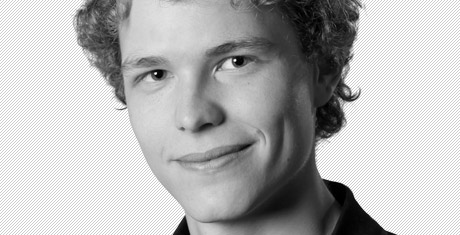
\includegraphics[width=10em]{peters.jpg}
%\end{minipage}
}
\title[Storage Solution for Models with Multiple Versions]{\Large Storage Solution for Models with Multiple Versions}
\subtitle{\small Concept and Prototype Implementation}


% ein alternatives Titelbild kann mittels 
%\titleimage{Dateiname.xyz}
% angegeben werden (auf vernuenftiges Seitenformat und Kontrastwerte achten, Skalierung und Abschneiden der oberen rechten Ecke passieren automatisch)
%\titleimage{scharm_02.jpg}
\titleimage{}
%%%%%%%%%%%% Festlegungen fuer Kopf- und Fusszeile %%%%%%%%%%%%%%%%%%%%
% Institutsname f\"ur die Fusszeile (nur wenn bei Paketeinbindung 'footuni' angegeben ist)
\footinstitute{Department of Systems Biology \& Bioinformatics\\Faculty of Computer Science \& Electrical Engineering}%Mathematisch-Naturwissenschaftliche Fakult\"at, Institut f\"ur Physik}
% eigenes Logo oben rechts hinzufuegen (bitte auf vernuenftiges Format achten - ein zu hohes Logo verschiebt das Layout)
\renewcommand{\mylogo}{
	%\hfill 
\includegraphics[height=8mm]{./unirostock/institutslogo}
	%\hfill 
\includegraphics[trim=22.2cm 0cm 0cm 8.6cm,clip=true,height=8mm]{./unirostock/sems_2}
}

\usepackage{listings}
\usepackage{tikz}
\usepackage{pgfplots}
\usetikzlibrary{shapes,arrows,trees,decorations.pathmorphing,backgrounds,fit}
 
\newcommand{\newsection}[1]{
\section{#1}
%\begin{frame}{#1}\tableofcontents[currentsection]\note{tof: #1}\end{frame}
}
\usepackage{tabularx}
\usepackage{wasysym}
\usepackage[misc]{ifsym}

\lstset{%
    %numbers=left,
    %numberstyle=\tiny\color{gray},
    %frame=tb
  }

% show other people's slides
\newenvironment{changemargin}[2]{%
\begin{list}{}{%
\setlength{\topsep}{0pt}%
\setlength{\leftmargin}{#1}%
\setlength{\rightmargin}{#2}%
\setlength{\listparindent}{\parindent}%
\setlength{\itemindent}{\parindent}%
\setlength{\parsep}{\parskip}%
}%
\item[]}{\end{list}}
\newcommand{\maxFrameImage}[2]{
\begin{frame}[plain]%
% \begin{tikzpicture}[overlay]%
% \draw[fill=red] (0,0) -- (-20,0) -- (-20,-20) -- (0,-20);%
% \end{tikzpicture}%
\begin{changemargin}{-1.45cm}{-1cm}
\begin{center}
\begin{tikzpicture}[overlay]
\fill[white] (-100,-100) rectangle (100,100);
\node[fill=white] (db4) at (0,-1) {\includegraphics[width=\paperwidth,height=\paperheight,keepaspectratio]{#1}};
\end{tikzpicture}
\end{center}#2
\end{changemargin}
\end{frame}
}

\usepackage{varwidth}

\definecolor{chck}{RGB}{0,155,85}



%
\pgfdeclaredecoration{penciline}{initial}{
    \state{initial}[width=+\pgfdecoratedinputsegmentremainingdistance,auto corner on length=9mm,]{
        \pgfpathcurveto%
        {% From
            \pgfqpoint{\pgfdecoratedinputsegmentremainingdistance}
                            {\pgfdecorationsegmentamplitude}
        }
        {%  Control 1
        \pgfmathrand
        \pgfpointadd{\pgfqpoint{\pgfdecoratedinputsegmentremainingdistance}{0pt}}
                        {\pgfqpoint{-\pgfdecorationsegmentaspect\pgfdecoratedinputsegmentremainingdistance}%
                                        {\pgfmathresult\pgfdecorationsegmentamplitude}
                        }
        }
        {%TO 
        \pgfpointadd{\pgfpointdecoratedinputsegmentlast}{\pgfpoint{1pt}{1pt}}
        }
    }
    \state{final}{}
}
\tikzset{pencila/.style={
    draw,
    decorate,
    decoration={random steps,segment length=3mm,amplitude=0.2mm}
  }
}
\tikzset{pencilb/.style={
    decorate,
    decoration={random steps,segment length=2pt,amplitude=0.3pt},
    to path={ -- ([xshift=rand*1mm, yshift=rand*1mm] \tikztotarget) \tikztonodes}
  }
}
\tikzset{pencilc/.style={
    decorate,
    decoration=penciline
  }
}
\tikzset{pencild/.style={
    draw,
    decorate,
    decoration={random steps,segment length=3.5mm,amplitude=0.1mm}
  }
}
\tikzset{trans/.style={->,pencilc,shorten >=1pt,shorten <=1pt,>=stealth,ultra thick,line width=.7mm,line cap=round
  }
}
\tikzset{bivesmapping/.style={-,pencilc,shorten >=3mm,shorten <=3mm,>=stealth,ultra thick,bivesmap,line cap=round
  }
}
\tikzset{annotation/.style={-,pencilc,shorten >=3mm,shorten <=1mm,>=stealth,ultra thick,gray,line cap=round
  }
}
\definecolor{dblue}{cmyk}{1.00, 0.75, 0.00, 0.00}

\newcommand{\changefont}[3]{\fontfamily{#1} \fontseries{#2} \fontshape{#3} \selectfont}

\usepackage{hyperxmp}
\hypersetup{
	pdfauthor={Martin Peters},
	pdfauthortitle={Bachelor Student},
	pdfcreator={},
	pdflang={en},
	pdfkeywords={SBML, CellML, BiVeS, MaSyMoS, Neo4j, graph database, database, version, model, Systems Biology},
	pdftype={Text},
	pdfcopyright={Copyright (C) 2016, Martin Peters. This work is licensed under a Creative Commons Attribution-ShareAlike 4.0 International License. (CC-BY-SA)},
	pdflicenseurl={http://creativecommons.org/licenses/by-sa/4.0/}
}

\renewcommand{\ttdefault}{pcr}
\newcommand{\twobar}{/\kern-0.2em/}

\pgfdeclarelayer{bg}    % declare background layer
\pgfsetlayers{bg,main} 


% beamer options regarding notes
%\setbeameroption{show only notes}
%%%%%%%%%%%%%%%%%% Los geht's %%%%%%%%%%%%%%%%%%%%%%%%%%%%%%%%%%%%%%%%%
%%%%%%%%%%%%%%%%%%%%%%%%%%%%%%%%%%%%%%%%%%%%%%%%%%%%%%%%%%%%%%%%%%%%%%%
\begin{document}

\begin{frame}{}{\mylogo}% Titelseite
	\titlepage
	\note{
	 	My name is Martin Peters.
	}
\end{frame}






%%%%%%%%%%%%%%%%%%%%%%%%%%%%%%%%%%%%%%%%%%%%%%%%%%%%%%%%%%%%%%%%%%%%%%%
%%%%%%%%%%%%%%%%%%%%%%%%%%%%%%%%%%%%%%%%%%%%%%%%%%%%%%%%%%%%%%%%%%%%%%%
 \begin{frame}{Table of contents}
   %\tableofcontents[pausesections]
   \tableofcontents
   \note{bla bla toc}
 \end{frame}
 
\newsection{Introduction}
\begin{frame}{short}{long}
	\centering
	
		
\end{frame}

\begin{comment}

\begin{frame}[t]{}{\mylogo}\vspace{-1em}
{\textcolor{colorscheme} {\textbf{That's it!}}}\\
\begin{tikzpicture}[>=stealth',trans/.style = {->,densely dashed,lightgray},shift={(-3,-3)},font=\small\selectfont]
\node[anchor=west] (sems) at (0,0) {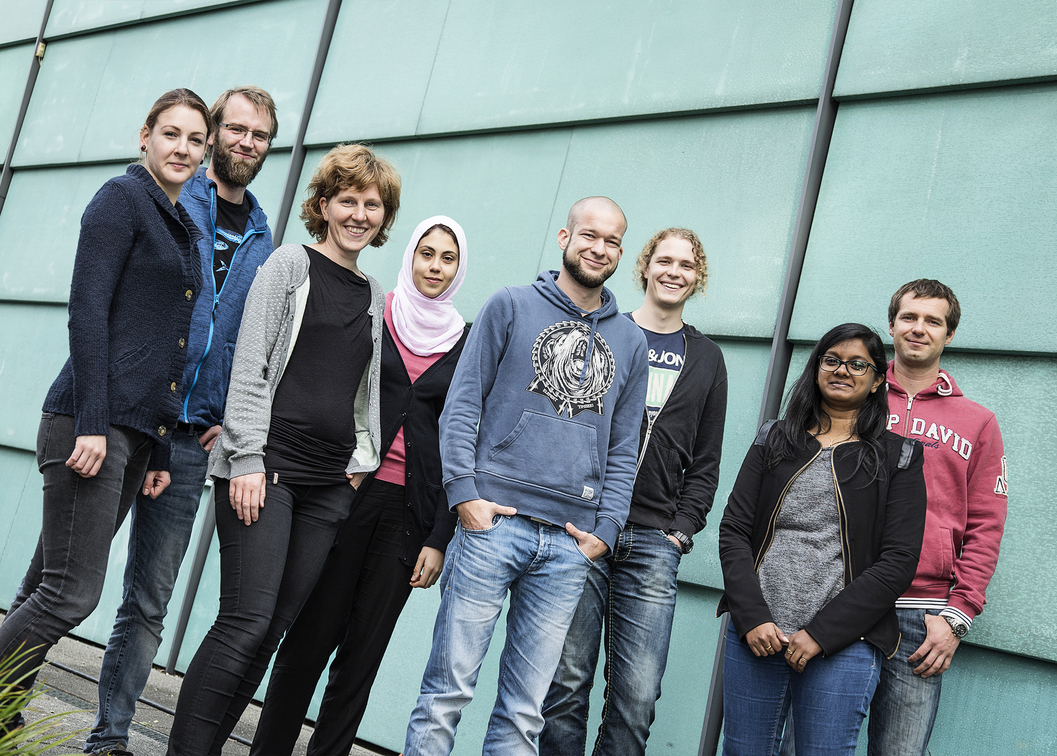
\includegraphics[height=.55\textheight]{res/group-2016.jpg}};
\node[anchor=west] (jws) at (4.9,0) {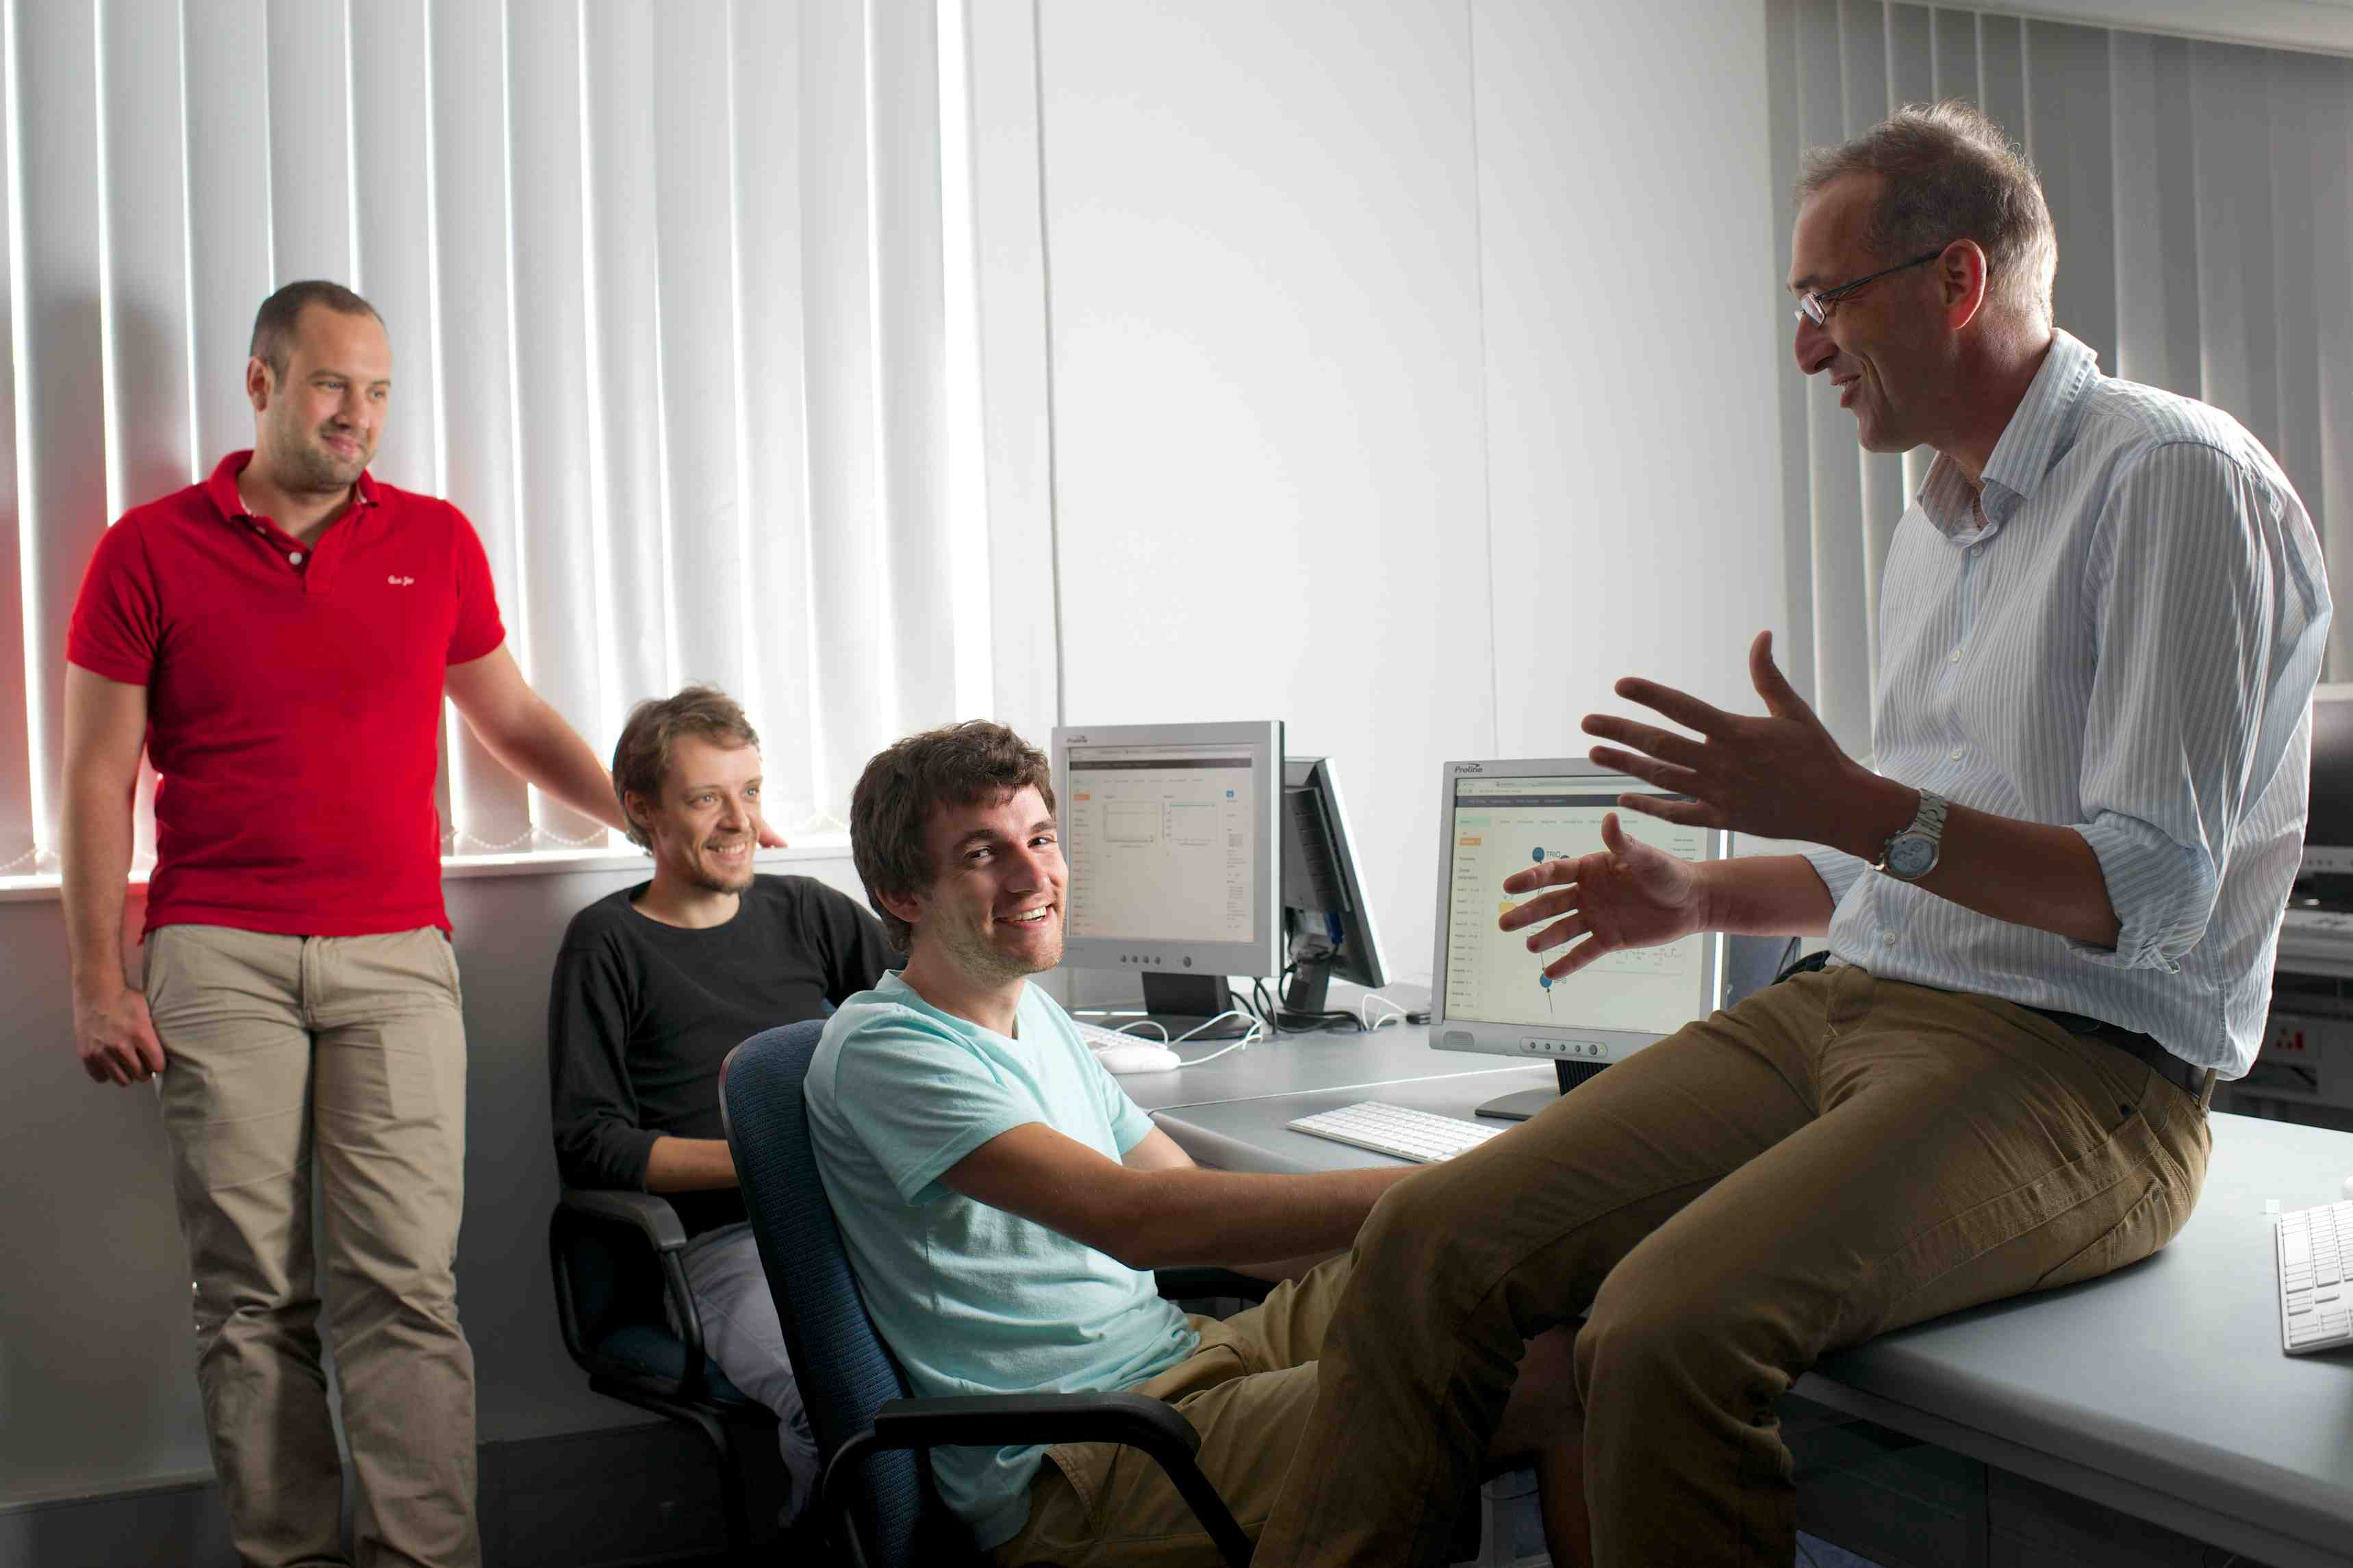
\includegraphics[height=.55\textheight]{res/jws_team.jpg}};
\node[yshift=-.1cm] at (sems.south) {SEMS Task Force};
\node[yshift=-.1cm] at (jws.south) {JWS Team};

\node[anchor=west] at (0, -3.45)  {
	\begin{minipage}[t][][t]{0.25\textwidth}
		\footnotesize
		Fabienne Lambusch\\
		Martin Scharm\\
		Dagmar Waltemath\\
		Mariam Nassar\\
	\end{minipage}
};

\node[anchor=west] at (2.7, -3.3)  {
	\begin{minipage}[t][][t]{0.25\textwidth}
		\footnotesize
		Tom Gebhardt\\
		%Martin Peters\\
		Vasundra Toure\\
		Ron Henkel\\
		Olaf Wolkenhauer
	\end{minipage}
};

\node[anchor=west] at (5.4, -3.32) {
	\begin{minipage}[t][][t]{0.25\textwidth}
		\footnotesize
		Dawie van Niekerk\\
		Johann Eicher\\
		Daniel Palm\\
		Jacky Snoep
	\end{minipage}
};

\node[anchor=west] at (9, -3.5) {
	\begin{minipage}[t][][t]{50pt}
		\hfill {\tiny funded by}\\
		\centering
		\includegraphics[width=50pt, height=2.5em, keepaspectratio]{res/BMBF-Logo.pdf}\\
		
\includegraphics[width=50pt, height=2.5em, keepaspectratio]{res/NRF_logo.jpg}
	\end{minipage}
};

\end{tikzpicture}

% % \scriptsize
% \begin{minipage}[t][.6\textheight][t]{.4\textwidth}
% %\vfil
% \quad\begin{tikzpicture}[overlay]
%  \node[rotate=90] at (-.5,-1.3) {SEMS Task Force};
%  \node[rotate=90] at (-.5,-4.3) {SBI Team};
% \end{tikzpicture}\\
% 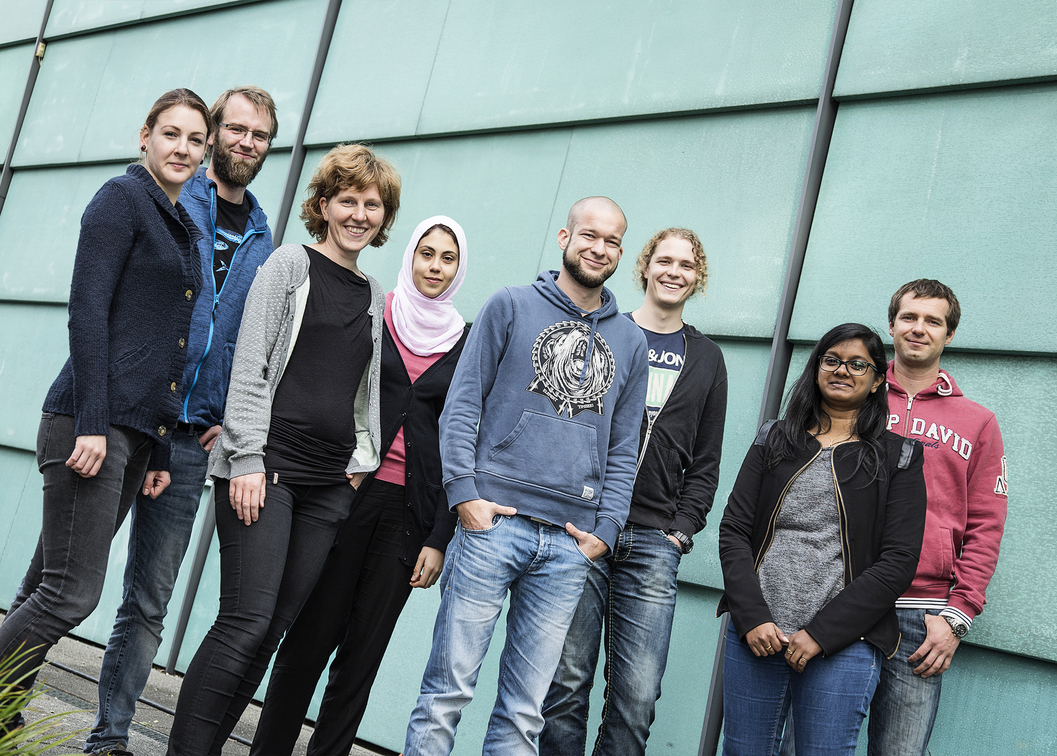
\includegraphics[width=.95\textwidth]{res/group-2016.jpg}\\[.5em]
% 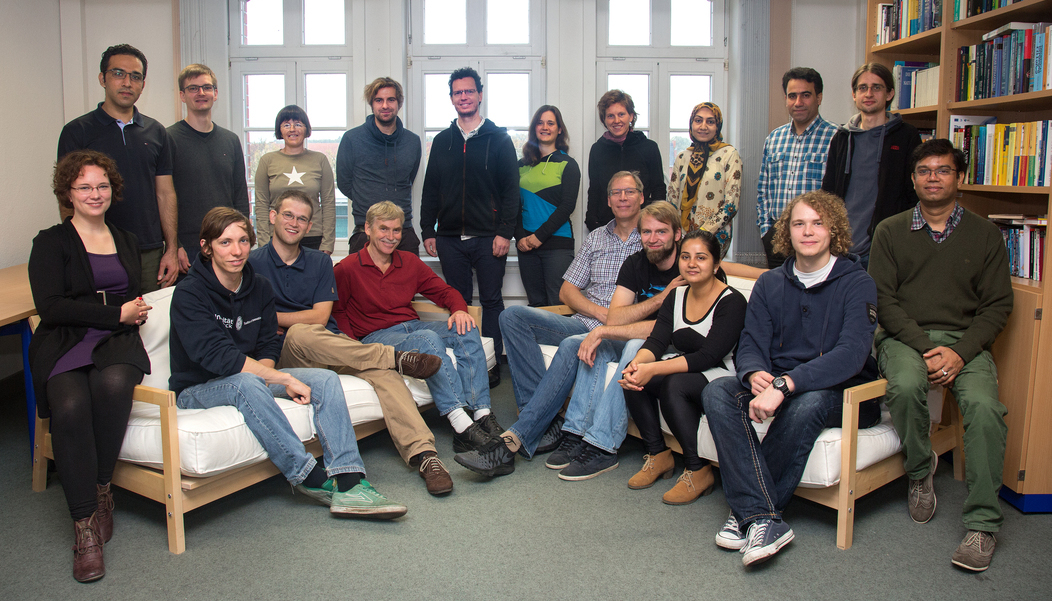
\includegraphics[width=.95\textwidth]{res/group-sbi.jpg}
% % \textbf{SEMS group}\\[.5em]
% % Dagmar Waltemath\\
% % Ron Henkel\\
% % Martin Peters\\
% % Markus Wolfien\\
% % Rebekka Alm\\
% % Olaf Wolkenhauer\\[1em]
% % \vfil
% % 
\includegraphics[height=1em]{res/twitter.png}\ \textcolor{colorscheme}{\tt\href{https://twitter.com/semsproject}{\small @SemsProject}}\\
% % \textcolor{colorscheme}{\tt\href{http://sems.uni-rostock.de}{\small http:\twobar{}sems.uni-rostock.de}}\\
% \vfil
% \end{minipage}
% % \hfill
% \begin{minipage}[t][.6\textheight][t]{.3\textwidth}
% % \vfil
% \quad\\
% % \textbf{SEMS group}\\[.5em]
% Tom Gebhardt\\
% Fabienne Lambusch\\
% Mariam Nassar\\
% Martin Peters\\
% Vasundra Toure\\
% Dagmar Waltemath\\
% Olaf Wolkenhauer
% % \textbf{SBI group}\\[.5em]
% % Olaf Wolkenhauer\\
% % Markus Wolfien
% \vfill
% \end{minipage}
% % \hfill
% \begin{minipage}[t][.6\textheight][t]{.29\textwidth}
% %\vfil
% %\textbf{Collaborators}\\[.5em]
% % Falk Schreiber\\
% % Jonathan Cooper (University of Oxford)\\
% % % COMBINE\\
% % \quad\\
% % 
\includegraphics[width=10em]{res/COMBINE.png}\\
% % 
\includegraphics[width=10em]{res/COMBINE.png}\\
% % 
\includegraphics[width=4em]{res/seek-logo-original.png}\hfill
% % 
\includegraphics[width=6em]{res/sysmodb2.png}\\
% % 
\includegraphics[width=5em]{res/bmdb.png}\hfill
% % \includegraphics[width=4em]{res/CellML-eps-converted-to.pdf}\\
% % \vfil
% \end{minipage}
% 
% \begin{flushright}
% 
\includegraphics[height=4em]{res/ptj-logo.png}\hspace{1em}\includegraphics[height=4em]{res/BMBF-Logo.pdf}%Logo_-_BMBF_19.png}
% \end{flushright}
% % \begin{tikzpicture}[overlay]
% % %  \node[red] at (2,4) {\LARGE reihenfolge? ich?};
% % %  \node[red] at (5,5) {\LARGE bild?};
% % %  \node[red] at (7,4) {\LARGE collaborators?};
% % \node[scale=.7] (combine) at (9,5.8) {
\includegraphics[width=10em]{res/COMBINE.png}};
% % \node[scale=.7] (bmdb) at (9.9,4.7) {
\includegraphics[width=4em]{res/seek-logo-original.png}};
% % \node[scale=.7] (sysmo) at (8.6,4.4) {
\includegraphics[width=6em]{res/sysmodb2.png}};
% % \node[scale=.7] (bmdb) at (9.9,3) {
\includegraphics[width=5em]{res/bmdb.png}};
% % \node[scale=.7] (pmr2) at (8.1,3.3) {\includegraphics[width=4em]{res/CellML-eps-converted-to.pdf}};
% % \end{tikzpicture}
\end{frame}


\end{comment}



 
\begin{frame}{}{\mylogo}
	{\LARGE That's it!}\\[1.05em]
	%{\Large Want to talk? Drop me a message!}
	%{\LARGE Thanks for your attention!}
	\\[1.4em]
	
	
\includegraphics[height=1em]{res/github.pdf}\ 
	Fork me on GitHub\\
	\textcolor{colorscheme}{\url{https://github.com/FreakyBytes/bachelor-thesis}}
	
	
\includegraphics[height=1em]{res/twitter.png}
	\textcolor{colorscheme}{\tt\  \href{https://twitter.com/FreakyBytes}{@FreakyBytes}}\\
	
	
\includegraphics[height=1em]{res/XMPP_logo.pdf}
	\textcolor{colorscheme}{\tt\  martin@freakybytes.net}\\
	
	\includegraphics[height=0.8em]{res/mail.pdf}
	\textcolor{colorscheme}{\tt\  martin.peters4@uni-rostock.de} 
	
	
\end{frame}

\begin{frame}{}{\mylogo}\vspace{-1em}
References
\footnotesize
%\tiny
%\small
\begin{itemize}
	\item ...
\end{itemize}

\end{frame}



%%%%%%%%%%%% Schluss jetzt %%%%%%%%%%%%%%%%%%%%%%%%%%%%%%%%%%%%%%%%%%%%
%%%%%%%%%%%%%%%%%%%%%%%%%%%%%%%%%%%%%%%%%%%%%%%%%%%%%%%%%%%%%%%%%%%%%%%
\end{document}

